\chapter{Planeación de acciones}
Un aspecto importante del comportamiento del robot en el contexto que se plantea es que le sea posible desarrollar una serie de actividades que en conjunto lleven a un resultado final.
Con este objetivo se desarrollaron varias máquinas de estados en los que la secuencia de acciones, así como las condiciones, variaban dependiendo del objetivo final. 
Dentro de los escenarios considerados se requiere lograr 3 tareas específicas, en las que progresivamente se añadían capacidades al desempeño del robot.

Como se mencionó en secciones anteriores, para el planteamiento de las máquinas de estado se necesita determinar las entradas, salidas, estados,  condiciones de transformación y las reglas de correspondencia que permiten el flujo de la información dentro de la secuencia de acciones.\\
En este caso, las entradas del sistema se refieren a la información que el robot es capaz de recopilar tanto de las condiciones de su ambiente como de su estado interno.
Haciendo uso de los sensores con que cuenta el robot puede determinar su posición respecto al mapa, y las posiciones también de los elementos en el entorno con los que debe interactuar.
Además, la información para el desarrollo de su actividad es previamente ingresada en una base de conocimiento de la cual el robot debe poder extraer la información y saber en qué parte de la secuencia de acciones se encuentra.

Es deseable que el robot cuente con estrategias que le permitan verificar si el estado en que el robot \textit{cree} que está es correcto y también comprobar que las acciones que se han registrado como realizadas se han completado correctamente.

\section{Actividades de la competencia RoboCup Logistics}
Como parte de las secciones que componen a la competencia \textit{RoboCup Logistics} se creó una categoría en la que se evalúan las diferentes habilidades que es indispensable que el robot tenga: \textbf{Navegación, Exploración y Manipulación}. De esta forma se facilita la integración y la evaluación del desempeño del robot en un entorno controlado para cada tarea, a continuación se incluye la descripción de cada una obtenida del reglamento de la competencia \cite{technical_committee_20122022_robocup_2022}.

\subsection{Navegación}
Para la evaluación de la Navegación se solicita que el robot \textit{visite} 12 puntos aleatorios dentro del espacio y permanecer en esa posición por al menos 5 segundos consecutivos, utilizando el menor tiempo posible y evadiendo obstáculos estáticos durante su desplazamiento.
Esta etapa podría considerarse la menos compleja dentro de las tres planteadas, pero es una actividad primordial dentro del desempeño del robot, dado que de no ser capaz de realizarla, no sería posible completar las siguientes.

\subsection{Exploración}
Durante la etapa de exploración se busca que el robot lleve a cabo una navegación autónoma, mientras realiza el procesamiento de la imagen capturada por su cámara para el reconocimiento de las estaciones de trabajo. Dicho reconocimiento se hace utilizando los códigos ARUCO que se encuentran en la base de las estaciones de trabajo. Además, el robot debe identificar el tipo de estación, la posición y orientación en que se encuentra cada estación y reportar la información.

\subsection{Manipulación}
En el caso de la manipulación, la posición inicial del robot se encuentra frente a una de las estaciones de trabajo. En la salida de la banda transportadora de la estación se encuentra una pieza que debe ser tomada por el manipulador. El robot debe trasladarse al otro lado de la estación y colocar la pieza en la entrada de la banda transportadora. Este proceso se repite 3 veces y dependiendo del nivel de dificultad que elija, se puede trabajar con una o más estaciones en las cuales se debe repetir el mismo procedimiento. 


\textcolor{green}{Breve descripción de las tareas y qué se necesita para resolverlas (navegación, localización, manipulación, reconocimiento de objetos, etc)}

\section{Máquinas de estados}
Una vez conocidos los requerimientos establecidos en el reglamento para considerar como exitosas estas tareas, se explicará a continuación cómo se realizó la implementación de las tareas haciendo uso de Máquinas de Estados Finitos.

\subsection{Estados}
Dentro de los Estados que se ejecutan dentro de los algoritmos se lleva a cabo las acciones por medio de las cuales se modifican las entradas y salidas del sistema, haciendo uso de las funciones que provocan cambios en el comportamiento del robot, de forma que se cumplan las condiciones de trancisión entre estados.

\subsection{Navegación}
La secuencia de Estados comienza con una etapa en la que se espera que el robot reciba el mensaje del sistema centralizado en el que se le indican las zonas del mapa que deben ser visitadas. Dado que se sabe el número específico de zonas necesarias para considerar la tarea como exitosa, el robot permanece en espera hasta que se completa el mensaje. 
Debido a que la información de las zonas objetivo se recibe como una cadena de texto, es necesario procesarla y se colocan los nombres en un arreglo desde el cual es más sencillo acceder a la información, además de conocer cuáles de los puntos ya han sido visitados y cuáles aún están pendientes. 
La condición de trancisión para este estado depende de la bandera \textbf{flag\_zones} mediante la cual se verifica que todas las zonas solicitadas se hayan visitado exitosamente, de lo contrario se sigue intentando, este proceso se repite hasta que se haya completado las zonas o bien se termine el tiempo permitido.
Con el arreglo de las zonas que se ha de visitar y sabiendo previamente las posiciones de las zonas en el mapa, se utiliza el algoritmo \textbf{Nearest Neighbour}, mediante el cual se calcula una ruta a seguir por el robot, buscando hacer el recorrido en el menor tiempo posible.
Cuando se cuenta con la ruta a seguir se utiliza la función \textbf{navigate\_to\_location}, con la cual el robot se desplaza hasta el centro de la zona solicitada. Se agrega un tiempo de espera para cumplir con los 5 segundos que se requieren para considerar la visita como exitosa y una vez pasado ese tiempo, se continúa con la ruta. Haciendo uso de la bandera \textbf{cont} se verifica el número de zonas visitadas y, en caso de haber completado las 12 zonas, se concluye la ejecución de la máquina de estados. 

\subsection{Exploración}
En el caso de la etapa de exploración, se consideró establecer una ruta a seguir utilizando puntos del mapa desde los cuales realizar el escaneo en busca de las estaciones de trabajo.

La ruta designada se compone por 8 \textit{Puntos de Inspección Principales} y 11 \textit{Puntos de Inspección Intermedios}. En cada uno de estos puntos robot hace una breve pausa y realiza un giro de 360 grados sobre su propio eje en 4 pasos, dando oportunidad a que la cámara RGBD encuentre los códigos de las estaciones, de ser visibles desde su posición, y los reporte. De acuerdo con las reglas de la competencia, el robot debe empezar en un punto específico, junto al borde inferior del mapa, a la izquierda o derecha dependiendo del equipo al que pertenezca. Por motivos de simplicidad, en la Figura \ref{fig:Route_Exploration} se muestra el proceso si el robot pertenece al equipo magenta.
Una vez que el robot ha salido de la zona designada se establecen como objetivo las coordenadas de la zona que se encuentra en la esquina inferior izquierda del mapa, señalizado en la Figura como el \textit{Punto de Inspección Principal 1}. 
Debido a que el mapa corresponde a un rectángulo de $14\times8$[m], y a que las zonas de descanso de los robots se encuentran en la arista inferior del mapa, se decidió dividirlo en dos regiones principales, cada una de $7\times7$, dentro de las cuales se realiza la trayectoria de exploración.  
Como se puede observar en la ilustración, en las secciones del recorrido que corresponden a las diagonales de cada mitad del mapa, se definieron 2 \textit{Puntos de Inspección Intermedios}, mientras que en las aristas se utiliza solo uno. 

De acuerdo con el reglamento, el posicionamiento de las estaciones en el mapa debe ser simétrico entre cada una de las mitades del mapa, por lo cual teniendo la información sobre las estaciones contenidas en una mitad es posible inferir las de la otra. Al llegar al \textit{Punto de Inspección Principal 4} se verifica si se han encontrado todas las estaciones necesarias. Sin embargo, en caso de que al terminar la ruta de exploración de la mitad izquierda no se hayan localizado todas las estaciones, se continúa con la secuencia en la mitad derecha en busca de la información restante. 

\begin{figure}[ht]
    \centering
    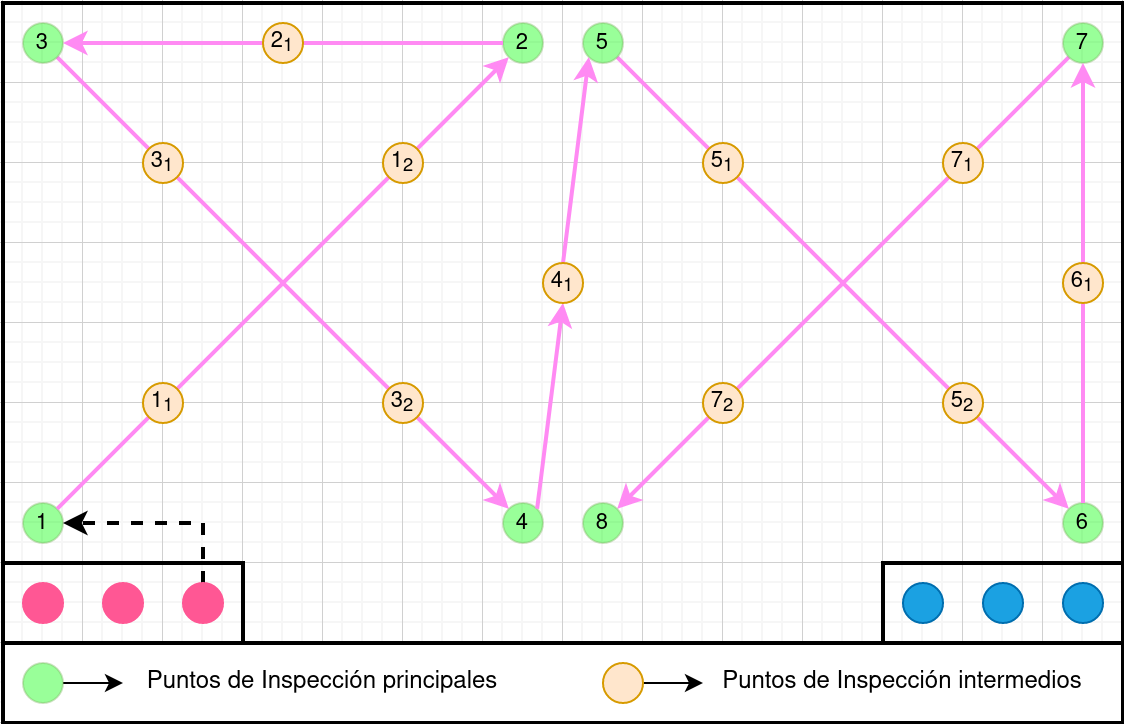
\includegraphics[scale= 0.3]{Figures/Exploration_route.png}
        \caption{Exploración}
        \label{fig:Route_Exploration}
    \end{figure}

Dentro de la Figura solo se muestran las rutas a seguir y los puntos de inspección que las componen, pero es importante recordar que las Estaciones de Trabajo que el robot está buscando representan también obstáculos estáticos dentro del entorno y que podrían interferir con la navegación del robot. Se sabe que el sistema de navegación que se está utilizando es un sistema confiable y robusto mediante el cual es posible realizar una navegación con evasión de obstáculos. 
No obstante, este es uno de los motivos por lo cual se consideró pertinente la definición de los puntos intermedios. Ya que si la navegación se ve interrumpida por  algún obstáculo y se excede el tiempo límite definido para dicha ruta, el sistema de navegación descarta esa coordenada y se define como objetivo el siguiente punto de inspección en la ruta. Adicionalmente, se definió que los puntos de inspección intermedios comprendieran perspectivas redundantes de algunas zonas, por lo que si los códigos en las paredes de las estaciones no son visibles desde un punto, es posible que lo sea desde otro.

\subsection{Manipulación}
Dentro de esta tarea, se aplican los conceptos mencionados en capítulos anteriores referentes al procesamiento de la imagen captada por la cárama RGBD.
Es en esta parte de la competencia en que se necesita identificar y localizar las piezas de interés dentro del espacio de trabajo del robot, tomarlas con el manipulador y transportarlas a otra ubicación determinada.
Para ello se solicita que el robot inicie el proceso frente a la MPS. Dadas las restricciones del dispositivo Kinect es necesario que el robot se encuentre a cierta distancia mínima del objeto de interés para obtener mediciones confiables del sensor del profundidad, por lo que de la posición inicial el robot debe retroceder un metro más. Es desde esta posición donde se ejecuta una función en la cual se utiliza la imagen RGB y se detectan las líneas contenidas en la Estación, excluyendo aquellas líneas que se sabe no pertenecen a la estación y aquellas que excedan un umbral del ángulo de inclinación, esta discriminación ayuda a disminuir el ruido de líneas detectadas por la cámara. Usando movimientos angulares de la base, se reduce el error entre el ángulo que se detecta del borde de la estación y una referencia horizontal definida empíricamente. Una vez que el robot está alineado se procede a la búsqueda del objeto sobre la superficie de la MPS.

Como se mencionó en capítulos anteriores, para la localización de las piezas se utilizó un algoritmo de segmentación por color de la imagen, una vez localizada, se le asigna una coordenada en el mapa relativa al origen del mismo. Dado que se cuenta ya con la información necesaria de la nube de puntos, y que la distancia que es posible alcanzar con el manipulador es limitada, el robot avanza la distancia que retrocedió anteriormente y se obtiene la transformación homogénea de la coordenada de la pieza con respecto a la posición actual del origen del manipulador del robot. Esta información es enviada al controlador del manipulador para calcular la trayectoria del mismo hacia la pieza. Dentro de la función que realiza esta acción, se posiciona la pinza frente a la coordenada solicitada, un par de centímetros antes, se abre la pinza, se realiza el desplazamiento hacia el frente para tomarla y finalmente se cierra la pinza. 

Una vez que la pieza se encuentra en el manipulador, el robot puede retroceder nuevamente y realizar la navegación hasta el punto de entrega (en el extremo opuesto de la MPS). Donde una vez más se utiliza el algoritmo de alineación y procesamiento de imagen para depositar la pieza sobre la banda transportadora. Suponiendo que se haya elegido un nivel de complejidad que involucre el uso de otra MPS, el robot realiza ahora la navegación y repite el proceso.

\subsection{Entradas y salidas}
Un elemento indispensable del comportamiento del robot depende de la información que recibe sobre su estado y el de su entorno.
\textbf{Localización} - El robot debe \textit{saber} su posición relativa al espacio en que se encuentra, esto, cuando es posible, se logra con un mapa previo del entorno en que se planea que el robot desempeñe sus actividades, y el cambio en su posición dentro del mapa se monitorea y actualiza constantemente mediante una combinación entre la odometría del robot y el algoritmo de localización de Monte Carlo, utilizando las lecturas que recibe del sensor de distancia que se encuentra en la  base del robot.
\textbf{Navegación} - El robot debe ser capaz de moverse dentro de su entorno, por lo que es necesaria la implementación de un algoritmo que le permita moverse de un punto a otro. Esta navegación se debe realizar sin colisionar con otros objetos en el espacio. En el sistema de navegación utilizado para este proyecto, desarrollado por el Laboratorio de Biorobótica de la Facultad e Ingniería de la UNAM y probado previamente en la liga @Home (tanto OpenPlatform como D) de la competencia RoboCup, se utilizan las lecturas del sensor de distancia, en conjunto con el algoritmo A* para realizar el cálculo de una ruta óptima entre dos puntos. 

\subsection{Algoritmos de las Máquinas de Estados - Cartas ASM}
A continuación se muestran los diagramas de flujo que representan el funcionamiento de las máquinas de estado utilizadas para cada actividad.

\begin{figure}[ht]
    \centering
    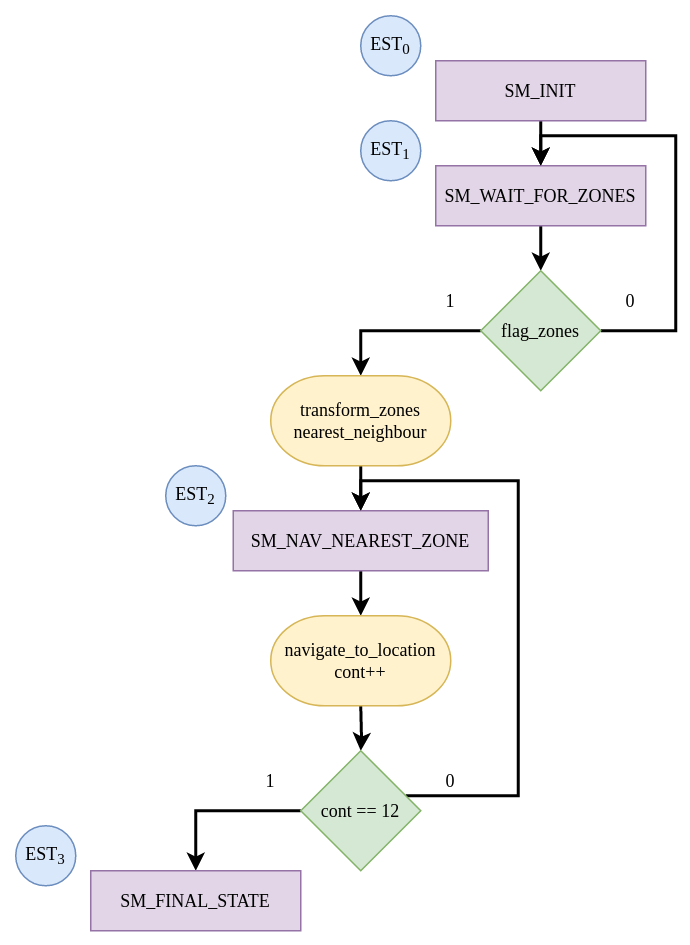
\includegraphics[scale= 0.4]{Figures/Navigation_CT.png}
        \caption{Navegación}
        \label{fig:ASM_Navigation}
    \end{figure}

\begin{figure}[ht]
    \centering
    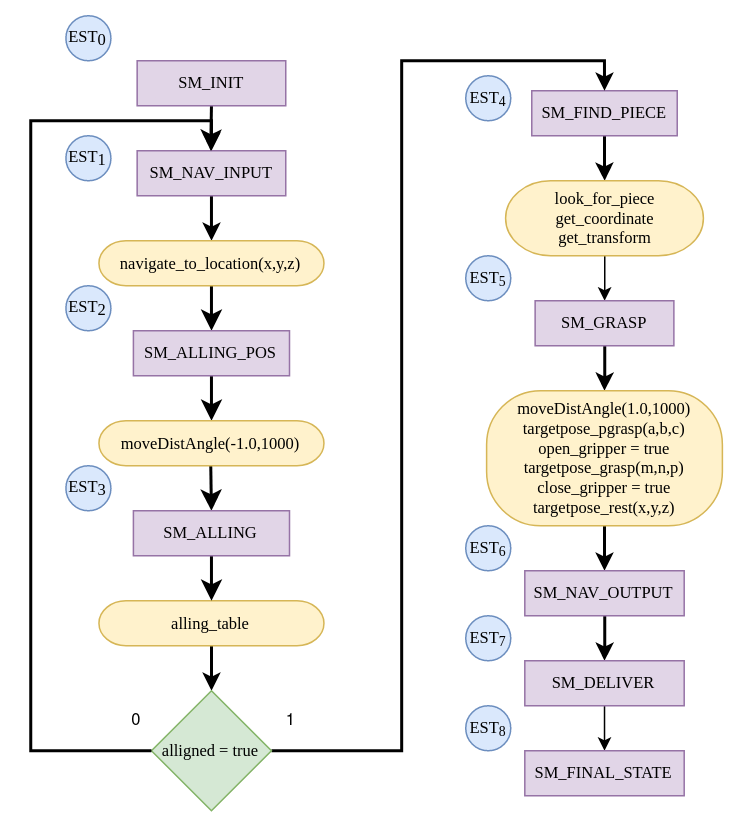
\includegraphics[scale= 0.5]{Figures/Manipulacion_CT_Hor.png}
    \caption{Manipulación}
    \label{fig:ASM_Manipulación}
\end{figure}

\subsection{Implementación}
Pseudocódigo de la implementación en C